% Options for packages loaded elsewhere
\PassOptionsToPackage{unicode}{hyperref}
\PassOptionsToPackage{hyphens}{url}
%
\documentclass[
  man,floatsintext]{apa6}
\usepackage{amsmath,amssymb}
\usepackage{iftex}
\ifPDFTeX
  \usepackage[T1]{fontenc}
  \usepackage[utf8]{inputenc}
  \usepackage{textcomp} % provide euro and other symbols
\else % if luatex or xetex
  \usepackage{unicode-math} % this also loads fontspec
  \defaultfontfeatures{Scale=MatchLowercase}
  \defaultfontfeatures[\rmfamily]{Ligatures=TeX,Scale=1}
\fi
\usepackage{lmodern}
\ifPDFTeX\else
  % xetex/luatex font selection
\fi
% Use upquote if available, for straight quotes in verbatim environments
\IfFileExists{upquote.sty}{\usepackage{upquote}}{}
\IfFileExists{microtype.sty}{% use microtype if available
  \usepackage[]{microtype}
  \UseMicrotypeSet[protrusion]{basicmath} % disable protrusion for tt fonts
}{}
\makeatletter
\@ifundefined{KOMAClassName}{% if non-KOMA class
  \IfFileExists{parskip.sty}{%
    \usepackage{parskip}
  }{% else
    \setlength{\parindent}{0pt}
    \setlength{\parskip}{6pt plus 2pt minus 1pt}}
}{% if KOMA class
  \KOMAoptions{parskip=half}}
\makeatother
\usepackage{xcolor}
\usepackage{graphicx}
\makeatletter
\def\maxwidth{\ifdim\Gin@nat@width>\linewidth\linewidth\else\Gin@nat@width\fi}
\def\maxheight{\ifdim\Gin@nat@height>\textheight\textheight\else\Gin@nat@height\fi}
\makeatother
% Scale images if necessary, so that they will not overflow the page
% margins by default, and it is still possible to overwrite the defaults
% using explicit options in \includegraphics[width, height, ...]{}
\setkeys{Gin}{width=\maxwidth,height=\maxheight,keepaspectratio}
% Set default figure placement to htbp
\makeatletter
\def\fps@figure{htbp}
\makeatother
\setlength{\emergencystretch}{3em} % prevent overfull lines
\providecommand{\tightlist}{%
  \setlength{\itemsep}{0pt}\setlength{\parskip}{0pt}}
\setcounter{secnumdepth}{-\maxdimen} % remove section numbering
% Make \paragraph and \subparagraph free-standing
\makeatletter
\ifx\paragraph\undefined\else
  \let\oldparagraph\paragraph
  \renewcommand{\paragraph}{
    \@ifstar
      \xxxParagraphStar
      \xxxParagraphNoStar
  }
  \newcommand{\xxxParagraphStar}[1]{\oldparagraph*{#1}\mbox{}}
  \newcommand{\xxxParagraphNoStar}[1]{\oldparagraph{#1}\mbox{}}
\fi
\ifx\subparagraph\undefined\else
  \let\oldsubparagraph\subparagraph
  \renewcommand{\subparagraph}{
    \@ifstar
      \xxxSubParagraphStar
      \xxxSubParagraphNoStar
  }
  \newcommand{\xxxSubParagraphStar}[1]{\oldsubparagraph*{#1}\mbox{}}
  \newcommand{\xxxSubParagraphNoStar}[1]{\oldsubparagraph{#1}\mbox{}}
\fi
\makeatother
% definitions for citeproc citations
\NewDocumentCommand\citeproctext{}{}
\NewDocumentCommand\citeproc{mm}{%
  \begingroup\def\citeproctext{#2}\cite{#1}\endgroup}
\makeatletter
 % allow citations to break across lines
 \let\@cite@ofmt\@firstofone
 % avoid brackets around text for \cite:
 \def\@biblabel#1{}
 \def\@cite#1#2{{#1\if@tempswa , #2\fi}}
\makeatother
\newlength{\cslhangindent}
\setlength{\cslhangindent}{1.5em}
\newlength{\csllabelwidth}
\setlength{\csllabelwidth}{3em}
\newenvironment{CSLReferences}[2] % #1 hanging-indent, #2 entry-spacing
 {\begin{list}{}{%
  \setlength{\itemindent}{0pt}
  \setlength{\leftmargin}{0pt}
  \setlength{\parsep}{0pt}
  % turn on hanging indent if param 1 is 1
  \ifodd #1
   \setlength{\leftmargin}{\cslhangindent}
   \setlength{\itemindent}{-1\cslhangindent}
  \fi
  % set entry spacing
  \setlength{\itemsep}{#2\baselineskip}}}
 {\end{list}}
\usepackage{calc}
\newcommand{\CSLBlock}[1]{\hfill\break\parbox[t]{\linewidth}{\strut\ignorespaces#1\strut}}
\newcommand{\CSLLeftMargin}[1]{\parbox[t]{\csllabelwidth}{\strut#1\strut}}
\newcommand{\CSLRightInline}[1]{\parbox[t]{\linewidth - \csllabelwidth}{\strut#1\strut}}
\newcommand{\CSLIndent}[1]{\hspace{\cslhangindent}#1}
\ifLuaTeX
\usepackage[bidi=basic]{babel}
\else
\usepackage[bidi=default]{babel}
\fi
\babelprovide[main,import]{english}
% get rid of language-specific shorthands (see #6817):
\let\LanguageShortHands\languageshorthands
\def\languageshorthands#1{}
% Manuscript styling
\usepackage{upgreek}
\captionsetup{font=singlespacing,justification=justified}

% Table formatting
\usepackage{longtable}
\usepackage{lscape}
% \usepackage[counterclockwise]{rotating}   % Landscape page setup for large tables
\usepackage{multirow}		% Table styling
\usepackage{tabularx}		% Control Column width
\usepackage[flushleft]{threeparttable}	% Allows for three part tables with a specified notes section
\usepackage{threeparttablex}            % Lets threeparttable work with longtable

% Create new environments so endfloat can handle them
% \newenvironment{ltable}
%   {\begin{landscape}\centering\begin{threeparttable}}
%   {\end{threeparttable}\end{landscape}}
\newenvironment{lltable}{\begin{landscape}\centering\begin{ThreePartTable}}{\end{ThreePartTable}\end{landscape}}

% Enables adjusting longtable caption width to table width
% Solution found at http://golatex.de/longtable-mit-caption-so-breit-wie-die-tabelle-t15767.html
\makeatletter
\newcommand\LastLTentrywidth{1em}
\newlength\longtablewidth
\setlength{\longtablewidth}{1in}
\newcommand{\getlongtablewidth}{\begingroup \ifcsname LT@\roman{LT@tables}\endcsname \global\longtablewidth=0pt \renewcommand{\LT@entry}[2]{\global\advance\longtablewidth by ##2\relax\gdef\LastLTentrywidth{##2}}\@nameuse{LT@\roman{LT@tables}} \fi \endgroup}

% \setlength{\parindent}{0.5in}
% \setlength{\parskip}{0pt plus 0pt minus 0pt}

% Overwrite redefinition of paragraph and subparagraph by the default LaTeX template
% See https://github.com/crsh/papaja/issues/292
\makeatletter
\renewcommand{\paragraph}{\@startsection{paragraph}{4}{\parindent}%
  {0\baselineskip \@plus 0.2ex \@minus 0.2ex}%
  {-1em}%
  {\normalfont\normalsize\bfseries\itshape\typesectitle}}

\renewcommand{\subparagraph}[1]{\@startsection{subparagraph}{5}{1em}%
  {0\baselineskip \@plus 0.2ex \@minus 0.2ex}%
  {-\z@\relax}%
  {\normalfont\normalsize\itshape\hspace{\parindent}{#1}\textit{\addperi}}{\relax}}
\makeatother

\makeatletter
\usepackage{etoolbox}
\patchcmd{\maketitle}
  {\section{\normalfont\normalsize\abstractname}}
  {\section*{\normalfont\normalsize\abstractname}}
  {}{\typeout{Failed to patch abstract.}}
\patchcmd{\maketitle}
  {\section{\protect\normalfont{\@title}}}
  {\section*{\protect\normalfont{\@title}}}
  {}{\typeout{Failed to patch title.}}
\makeatother

\usepackage{xpatch}
\makeatletter
\xapptocmd\appendix
  {\xapptocmd\section
    {\addcontentsline{toc}{section}{\appendixname\ifoneappendix\else~\theappendix\fi: #1}}
    {}{\InnerPatchFailed}%
  }
{}{\PatchFailed}
\makeatother
\usepackage{csquotes}
\ifLuaTeX
  \usepackage{selnolig}  % disable illegal ligatures
\fi
\usepackage{bookmark}
\IfFileExists{xurl.sty}{\usepackage{xurl}}{} % add URL line breaks if available
\urlstyle{same}
\hypersetup{
  pdftitle={ChildLens: An Egocentric Video Dataset for Activity Analysis in Children},
  pdfauthor={Nele-Pauline Suffo1, Pierre-Etienne Martin2, Daniel Haun2, \& Manuel Bohn1, 2},
  pdflang={en-EN},
  hidelinks,
  pdfcreator={LaTeX via pandoc}}

\title{ChildLens: An Egocentric Video Dataset for Activity Analysis in Children}
\author{Nele-Pauline Suffo\textsuperscript{1}, Pierre-Etienne Martin\textsuperscript{2}, Daniel Haun\textsuperscript{2}, \& Manuel Bohn\textsuperscript{1, 2}}
\date{}


\shorttitle{ChildLens Dataset}

\authornote{

The authors made the following contributions. Nele-Pauline Suffo: Conceptualization, Writing - Original Draft Preparation, Writing - Review \& Editing; Manuel Bohn: Writing - Review \& Editing, Supervision.

Correspondence concerning this article should be addressed to Nele-Pauline Suffo, Universitätsallee 1, 21335 Lüneburg. E-mail: \href{mailto:nele.suffo@leuphana.de}{\nolinkurl{nele.suffo@leuphana.de}}

}

\affiliation{\vspace{0.5cm}\textsuperscript{1} Institute of Psychology in Education, Leuphana University Lüneburg\\\textsuperscript{2} Max Planck Institute for Evolutionary Anthropology}

\abstract{%
One or two sentences providing a \textbf{basic introduction} to the field, comprehensible to a scientist in any discipline.
Two to three sentences of \textbf{more detailed background}, comprehensible to scientists in related disciplines.
One sentence clearly stating the \textbf{general problem} being addressed by this particular study.
One sentence summarizing the main result (with the words ``\textbf{here we show}'' or their equivalent).
Two or three sentences explaining what the \textbf{main result} reveals in direct comparison to what was thought to be the case previously, or how the main result adds to previous knowledge.
One or two sentences to put the results into a more \textbf{general context}.
Two or three sentences to provide a \textbf{broader perspective}, readily comprehensible to a scientist in any discipline.
}



\begin{document}
\maketitle

\section{Introduction}\label{introduction}

Lorem ipsum dolor sit amet, consectetur adipiscing elit. Sed ac purus sit amet nisl tincidunt tincidunt. Nullam nec turpis at libero tincidunt tincidunt. Sed nec mi nec nunc tincidunt tincidunt. Nullam nec turpis at libero tincidunt tincidunt. Sed nec mi nec nunc

\section{Dataset Overview}\label{dataset-overview}

\paragraph{Activity Classes}\label{activity-classes}

The ChildLens dataset contains a total of 14 activity and 5 location classes. The activities are based on the actions of the child in the video and can be divided into \emph{person-only} activities, such as ``child talking'' or ``other person talking, and \emph{person-object} activities, such as''drawing'' or ``playing with object''. You can find the complete list of activity classes with a brief description in the appendix. The activities can be further divided into \emph{audio-based}, \emph{visual-based}, and \emph{multimodal} activities, as presented in \ref{fig:activity-classes}. The following list provides an overview of the different activity types:

\begin{itemize}
\tightlist
\item
  \textbf{Audio-based activities}: \emph{child talking}, \emph{other person talking}, \emph{overheard speech}, \emph{singing / humming}, \emph{listening to music / audiobook}
\item
  \textbf{Visual-based activities}: \emph{watching something}, \emph{drawing}, \emph{crafting things}, \emph{dancing}
\item
  \textbf{Multimodal activities}: \emph{playing with object}, \emph{playing without object}, \emph{pretend play}, \emph{reading book}, \emph{making music}
\end{itemize}

The location classes describe the current location of the child in the video and include \emph{livingroom}, \emph{playroom}, \emph{bathroom}, \emph{hallway}, and \emph{other}.

\begin{figure}

{\centering 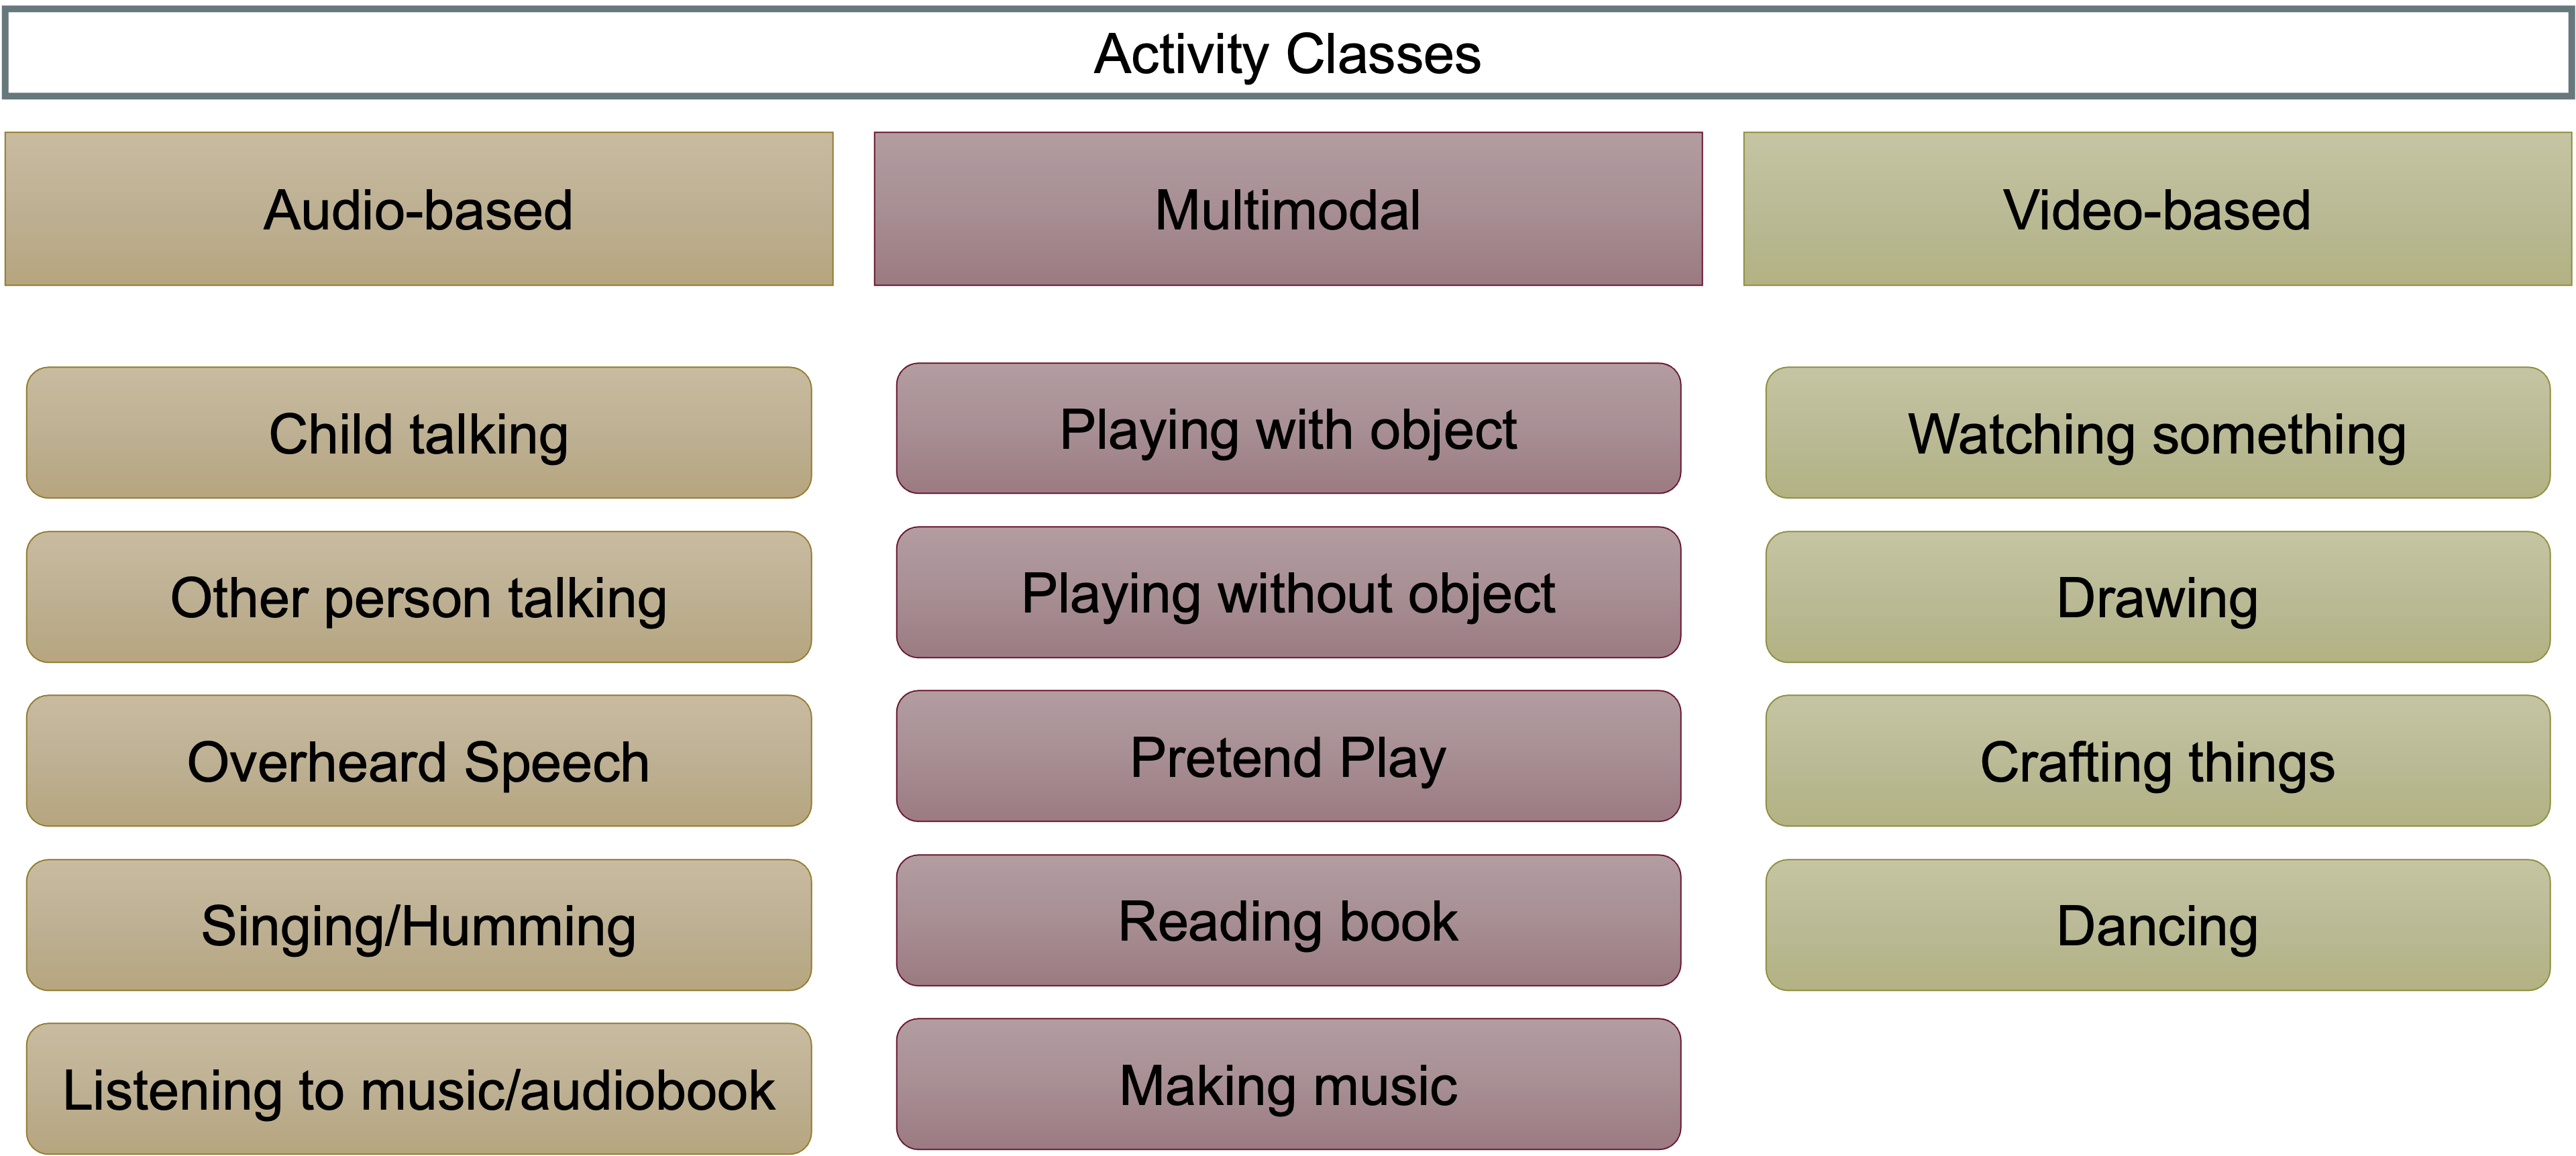
\includegraphics[width=5.95in]{activity_classes} 

}

\caption{ChildLens Activity Class Categories}\label{fig:activity-classes}
\end{figure}

\paragraph{Statistics}\label{statistics}

We have varying numbers of clips for each of the 14 activity classes, ranging from \emph{x} to \emph{x} clips per class. The duration of the clips differs depending on the activity; for example, audio-related actions like ``child talking'' may only last a few seconds, while activities like ``reading a book'' may last several minutes. The xxx video clips are divided into \emph{xx-xx } training clips, *xx** validation clips, and \emph{xx} testing clips for each class. Table \ref{tab:train-val-test} provides an overview of the numbers.

\begin{table}[tbp]

\begin{center}
\begin{threeparttable}

\caption{\label{tab:train-val-test}Number of clips per class}

\begin{tabular}{lll}
\toprule
training & \multicolumn{1}{c}{validation} & \multicolumn{1}{c}{testing}\\
\midrule
10 & 10 & 10\\
\bottomrule
\end{tabular}

\end{threeparttable}
\end{center}

\end{table}

\paragraph{Exhaustive multi-label annotations}\label{exhaustive-multi-label-annotations}

The dataset provides detailed annotations for each video file. These annotations specify the child's current location within the video, the start and end times of each activity, the activity class, and whether the child is engaged alone or with somebody else. For every person involved in the activity, we capture age and gender. If multiple activities occur simultaneously in a video, each activity is individually labeled and extracted as a separate clip. For example, if a segment shows a child ``reading a book'' while also ``talking,'' two separate clips are created: one for ``reading a book'' and another for ``child talking.'' This exhaustive labeling strategy ensures that each activity is accurately represented in the dataset. Figure \ref{fig:superannotate} provides a screenshot of the SuperAnnotate platform used for video annotation.

\begin{figure}

{\centering 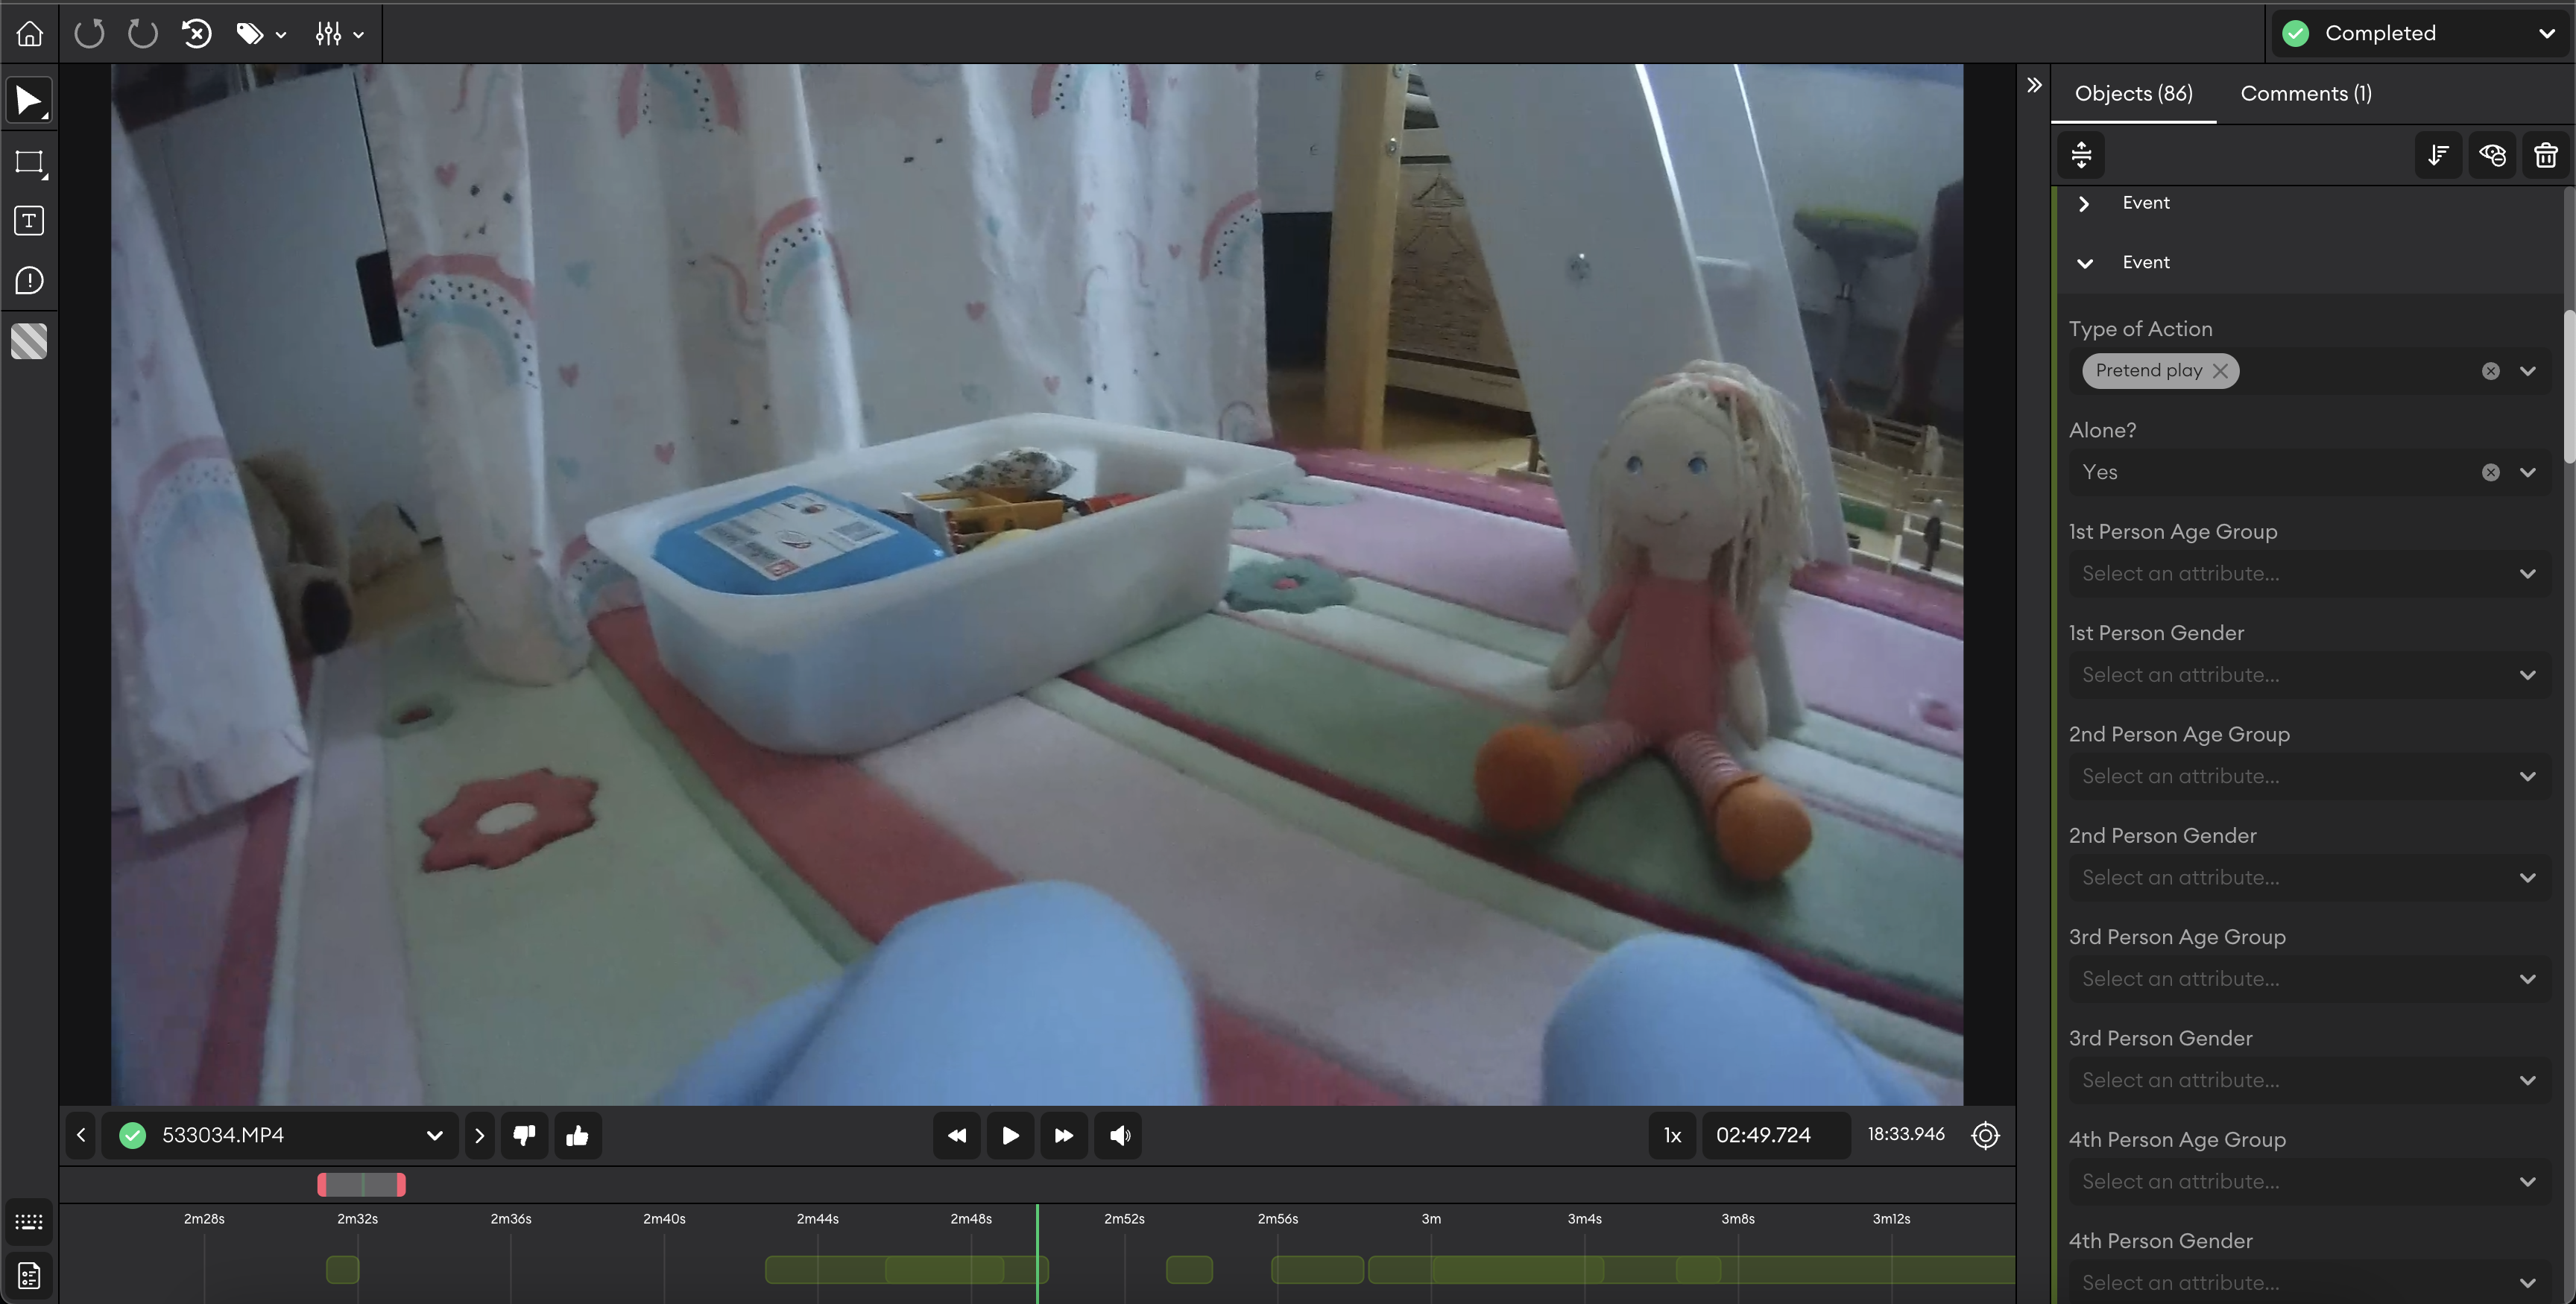
\includegraphics[width=5.76in]{SuperAnnotate} 

}

\caption{SuperAnnotate platform utilized for video annotation}\label{fig:superannotate}
\end{figure}

\section{Dataset Generation}\label{dataset-generation}

This section outlines the steps taken to create the ChildLens dataset. We provide detailed information on the video collection process, the labeling strategy employed, and the generation of activity labels.

\subsection{Step 1: Collection of Egocentric Videos}\label{step-1-collection-of-egocentric-videos}

The ChildLens dataset consists of egocentric videos recorded by children aged 3 to 5 years. A total of xx children from families living in a mid-sized city in Germany, participated in the study. The videos were captured at home using a camera embedded in a vest worn by the children, which can be seen in figure \ref{fig:camera-worn}. This setup allowed the children to move freely throughout their homes while recording their activities. The camera, a \emph{PatrolEyes WiFi HD Infrared Police Body Camera}, was equipped with a 140-degree wide-angle lens and captured everything within the child's field of view with a resolution of 1920x1080p at 30 fps. The camera also recorded audio, allowing us to capture the child's speech and other sounds in the environment. Additionally, the parents were handed a small checklist of activities to record, ensuring that a variety of activities were captured in the videos. The focus was on capturing everyday activities that children typically engage in. Parents were therefore asked to include the following activities in the recordings:
- Child is invited to read a book together with an adult
- Child is invited to play with toys alone
- Child is invited to play with toys with someone else (adult or child)
- Child is invited to draw/craft something

The videos were recorded over a period of xx months, resulting in a total of xx hours of video footage.

\begin{figure}

{\centering 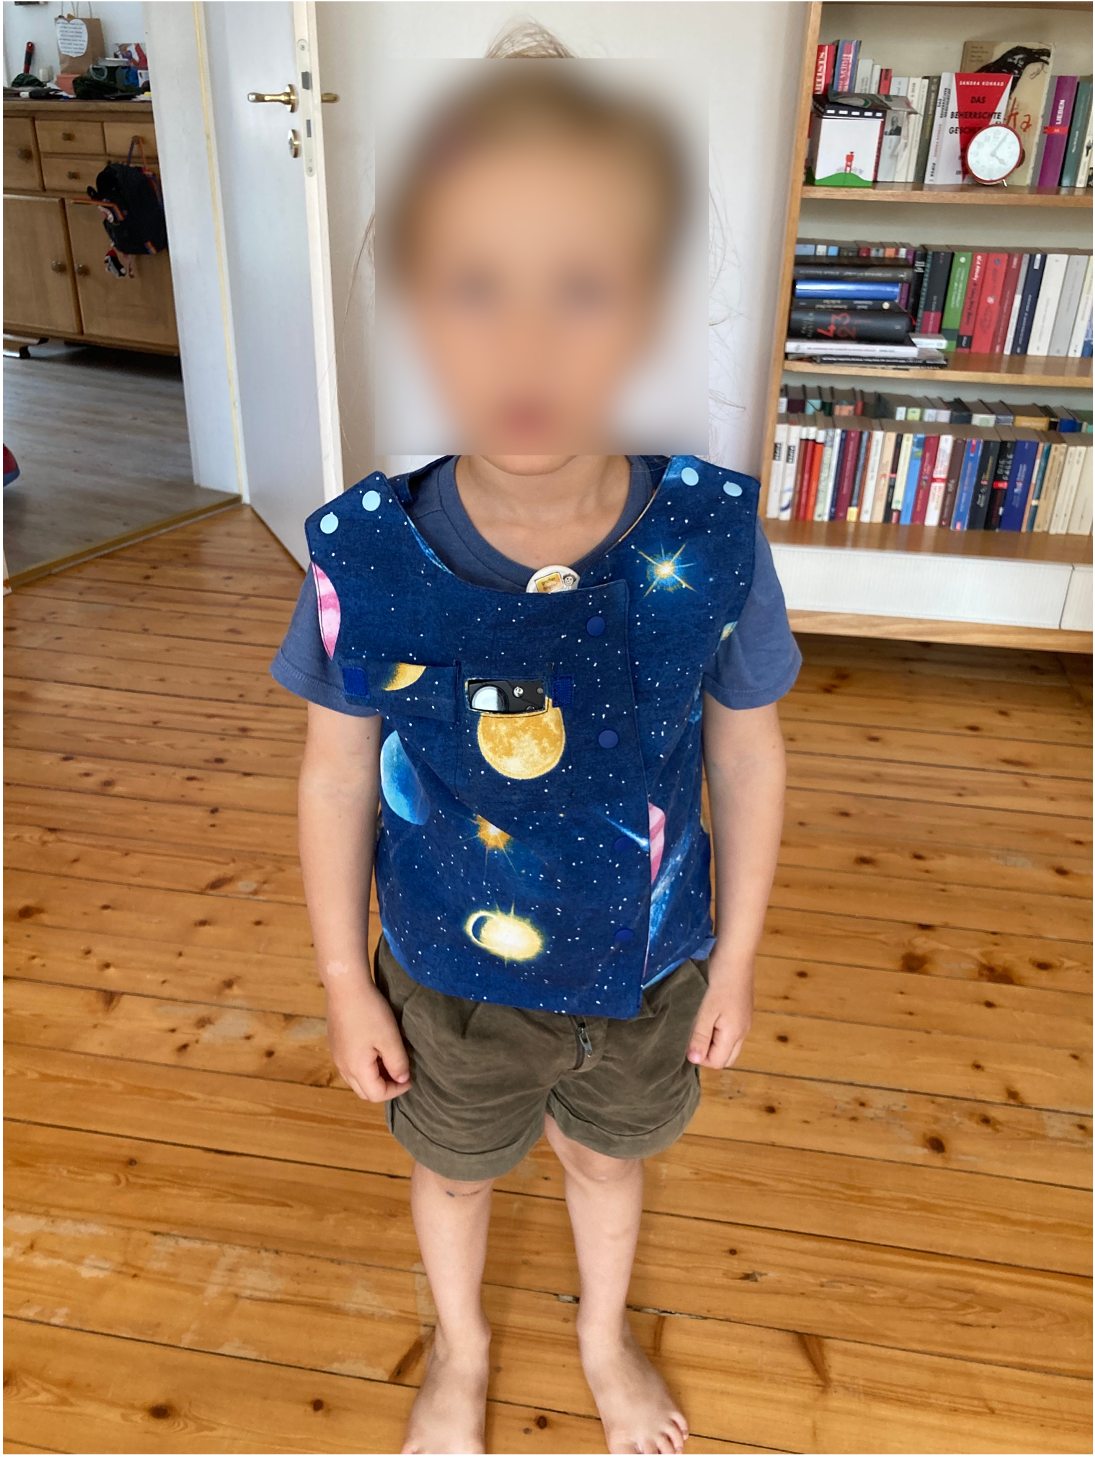
\includegraphics[width=2.19in]{camera_worn} 

}

\caption{Vest with the embedded camera worn by the children}\label{fig:camera-worn}
\end{figure}

\subsection{Step 2: Creation of Labeling Strategy}\label{step-2-creation-of-labeling-strategy}

After an initial review of the videos, we identified the most common activities that children engage in throughout the day. The activity classes in the dataset are derived from these activities. We chose to differentiate, for example, between ``drawing'' and ``crafting things'' or ``making music'' and ``singing/humming'' in order to make the activities more granular. We also added the concepts of ``overheard speech'', which describes situations in which the child is not directly involved in a conversation but can hear it, and ``pretend play'', which refers to when the child is engaged in imaginative play. This approach allowed us to capture the diversity of activities that children engage in and create a comprehensive dataset for activity analysis.

\subsection{Step 3: Manual Labeling Process}\label{step-3-manual-labeling-process}

The videos were manually annotated by native German speakers who watched each video and labeled the activities present in the footage. The annotators marked the start and end points of each activity, ensuring that the annotations were accurate and detailed. The labeling process was conducted using the SuperAnnotate platform, which allowed for efficient annotation and review of the videos.

\begin{itemize}
\item
  labeling process means looking at the whole video and mark start and end point of each activity present in the list of activities
\item
  we annotate the videos using humans
\item
  native germans for labeling task
\item
  use SuperAnnotate platform for labeling
\item
  review system: always two annotators label the same video,
  *-TODO: ask how exactly the review process works
\item
  in setup meeting we discussed the labeling strategy and the classes and handed over the annotation strategy to the annotators
\item
  before starting annotation process, we made sure that all questions were answered and that the annotators understood the task
\item
  before the actual annotation process started, the annotators labeled 25 videos to get a feeling for the task
\item
  the annotations then were reviewed by us and feedback was shared
\item
  in total three feedback loops were conducted to ensure that the annotators followed the labeling strategy
\end{itemize}

\section{Benchmark Performance}\label{benchmark-performance}

\subsection{Implementation details}\label{implementation-details}

\subsection{Boundary-Matching Network}\label{boundary-matching-network}

We utilize the BMN model (Lin, Liu, Li, Ding, \& Wen, 2019) for temporal activity localization.

\subsection{VTC}\label{vtc}

For the visual-based activities, we use the Voice Type Classifier (Lavechin, Bousbib, Bredin, Dupoux, \& Cristia, 2020).

\section{Conclusion}\label{conclusion}

\section{Discussion}\label{discussion}

\subsection{Dataset bias}\label{dataset-bias}

\subsection{General Discussion}\label{general-discussion}

\newpage

\section{References}\label{references}

\begingroup
\setlength{\parindent}{-0.5in}
\setlength{\leftskip}{0.5in}

\phantomsection\label{refs}
\begin{CSLReferences}{1}{0}
\bibitem[\citeproctext]{ref-lavechinOpensourceVoiceType2020}
Lavechin, M., Bousbib, R., Bredin, H., Dupoux, E., \& Cristia, A. (2020). \emph{An open-source voice type classifier for child-centered daylong recordings}. arXiv. \url{https://doi.org/10.48550/ARXIV.2005.12656}

\bibitem[\citeproctext]{ref-linBMNBoundaryMatchingNetwork2019}
Lin, T., Liu, X., Li, X., Ding, E., \& Wen, S. (2019). \emph{{BMN}: {Boundary-Matching Network} for {Temporal Action Proposal Generation}}. arXiv. \url{https://doi.org/10.48550/ARXIV.1907.09702}

\end{CSLReferences}

\endgroup

\newpage

\section{Appendix}\label{appendix}

\subsection{List of ChildLens Activity Classes}\label{list-of-childlens-activity-classes}

The dataset contains the following list of activities. The number of clips for each activity class is indicated by the number in brackets behind each class.

\begin{enumerate}
\def\labelenumi{\arabic{enumi}.}
\tightlist
\item
  \textbf{playing with object}: The child is playing with an object, such as a toy or a ball. (x clips)
\item
  \textbf{playing without object}: The child is playing without an object, such as playing hide and seek or catch. (x clips)
\item
  \textbf{pretend play}: The child is engaged in imaginative play, such as pretending to be a doctor or a firefighter. (x clips)
\item
  \textbf{watching something}: The child is watching a movie, TV show, or video on either a screen or a device. (x clips)
\item
  \textbf{reading book}: The child is reading a book or looking at pictures in a book (x clips)
\item
  \textbf{child talking}: The child is talking to themselves or to someone else (x clips)
\item
  \textbf{other person talking}: Another person is talking to the child. (x clips)
\item
  \textbf{overheard speech}: Conversations that the child can hear but is not directly involved in. (x clips)
\item
  \textbf{drawing}: The child is drawing or coloring a picture. (x clips)
\item
  \textbf{crafting things}: The child is engaged in a craft activity, such as making a bracelet or decoration. (x clips)
\item
  \textbf{singing / humming}: The child is singing or humming a song or a mekody. (x clips)
\item
  \textbf{making music}: The child is playing a musical instrument or making music in another way (x clips)
\item
  \textbf{dancing}: The child is dancing to music or moving to a rhythm. (x clips)
\item
  \textbf{listening to music / audiobook}: The child is listening to music or an audiobook. (x clips)
\end{enumerate}

\subsection{List of ChildLens Location Classes}\label{list-of-childlens-location-classes}

\begin{enumerate}
\def\labelenumi{\arabic{enumi}.}
\tightlist
\item
  livingroom
\item
  playroom
\item
  bathroom
\item
  hallawy
\item
  other
\end{enumerate}


\end{document}
